\documentclass[11pt,a4paper]{article}
\usepackage[utf8]{inputenc}
\usepackage[T1]{fontenc}
\usepackage{lmodern}
\usepackage[english]{babel}
\usepackage{microtype}
\usepackage[a4paper,margin=2.3cm]{geometry}
\usepackage{graphicx}
\usepackage{booktabs}
\usepackage{xcolor}
\usepackage{titlesec}
\usepackage{enumitem}
\usepackage{float}
\usepackage[hidelinks]{hyperref}
\definecolor{accent}{HTML}{1F4E79}
\titleformat{\section}{\large\bfseries\color{accent}}{\thesection}{0.6em}{}
\titleformat{\subsection}{\normalsize\bfseries}{\thesubsection}{0.6em}{}
\setlist{itemsep=2pt,topsep=3pt}
\setlength{\parskip}{4pt}
\graphicspath{{../figures/}}

\begin{document}

\begin{center}
{\LARGE\bfseries\color{accent} What France reimburses}\\[4pt]
{\large Medicines dispensed by retail pharmacies, 2019--2025}\\[8pt]
Deo Gratias Loutou \,\textbar\, \href{https://github.com/LDGKM/medicine-spending-france}{github.com/LDGKM/medicine-spending-france} \,\textbar\, October 2026
\end{center}

\section*{Executive summary}
French health insurance reimbursed \textbf{\texteuro 27.4 billion} of medicines dispensed by retail pharmacies in
2025, against \texteuro 19.1 billion in 2019: \textbf{+43\% in six years}. Yet the number of boxes dispensed did not
change (+1\%). The whole increase comes from \emph{what} is dispensed, not \emph{how much}: the average box rose from
\texteuro 9.77 to \texteuro 13.51.
\begin{itemize}
  \item \textbf{Innovative, expensive drugs drive the growth.} Cancer and immunology medicines explain \texteuro 3.2
        billion of the \texteuro 8.3 billion increase. A single molecule, tafamidis (a treatment for a rare heart
        disease), went from \texteuro 45 million to \texteuro 1.07 billion and is now the most reimbursed, for about
        16{,}000 patients.
  \item \textbf{Spending is concentrating}: 55 molecules out of about 1{,}100 make up half of the total (70 in 2019).
  \item \textbf{Three shifts in use}: patients on GLP-1 analogues (diabetes) more than doubled (415{,}000 to 932{,}000);
        antibiotic use collapsed during the pandemic and recovered by 2024; adults treated for ADHD with methylphenidate
        rose from 17{,}000 to 114{,}000.
  \item \textbf{Regions must be compared at equal age}: people over 60 cost almost eight times more per head than under-20s. After
        standardising for age, Île-de-France moves from 11th to 3rd of 12 regions; Grand Est ranks 4th.
\end{itemize}

\section{Question and data}
\textbf{Questions.} How fast is spending on medicines growing, and why? Which drugs and therapeutic areas drive it?
How has use changed for a few public-health topics? How do regions compare once age is taken into account?

\textbf{Data.} \emph{Open Medic}, published by the French national health insurance (Assurance Maladie) from the
national health data system (SNDS). It covers every box of medicine dispensed by a retail pharmacy and reimbursed by any
scheme, in mainland France and overseas; hospital medicines are not included and amounts exclude pharmacists' dispensing
fees. We use the ``NB'' files, which also count \emph{patients} (people who received the drug at least once in the year),
for 2019--2025, at three levels of the WHO Anatomical Therapeutic Chemical (ATC) classification:

\begin{table}[H]\centering\small
\begin{tabular}{llrl}\toprule
Level & Example & Rows & Use \\\midrule
ATC5 (molecule) & A10BJ06 semaglutide & 500{,}177 & spending by molecule, groups (first letter) \\
ATC4 (class) & A10BJ GLP-1 analogues & 225{,}025 & patients in a class, without double counting \\
ATC2 (group) & J01 antibacterials & 51{,}963 & patients on antibiotics \\\bottomrule
\end{tabular}
\caption{Each row: year $\times$ code $\times$ age group (0--19, 20--59, 60+) $\times$ sex $\times$ region of residence.}
\end{table}
Population: INSEE estimates on 1~January (2019--2023) by region, sex and age; 2023 is reused for 2024 and 2025.

\section{Method}
\textbf{Loading and cleaning.} Numbers are written in French format (\texttt{1.171,74} = 1171.74), converted by a SQL macro.
The files do not share an encoding (Windows-1252 for the class-level files of 2019--2024, UTF-8 for 2025), so every file
is first rewritten in UTF-8, then loaded into DuckDB.

\textbf{Validation.} Total spending computed from the molecule, class and group files is identical each year (to the euro),
and fewer than 0.2\% of euros have an unknown age, sex or label. 6.4\% of spending is attached to codes that are not
metropolitan regions (unknown residence or overseas); these are excluded from the regional comparison only.

\textbf{Stable molecules.} A molecule does not always keep the same code: the WHO moved GLP-1 analogues from A10BX to
A10BJ in 2020 and reorganised cancer drugs (L01XE $\rightarrow$ L01E\ldots) in 2021; some labels are also misspelt in
some years (``dapaglifozine''). Comparing codes over time would show these drugs as disappearing and new ones appearing.
We link two (code, label) pairs when they share the code \emph{or} the normalised label, and treat each connected group
as one molecule (union-find algorithm). This concerns 19\% of spending.

\textbf{Patients are not additive.} Someone taking two GLP-1 drugs is counted once per molecule. Class-level patient
numbers therefore come from the class-level file, never from adding molecules.

\textbf{Fair regional comparison.} Spending depends strongly on age. We use direct age standardisation: each region's
spending per inhabitant in each age group is weighted by the national age structure. With only three age groups the
adjustment is coarse but captures the main effect.

\section{Findings}
\subsection{Spending rises, volume does not}
\begin{figure}[H]\centering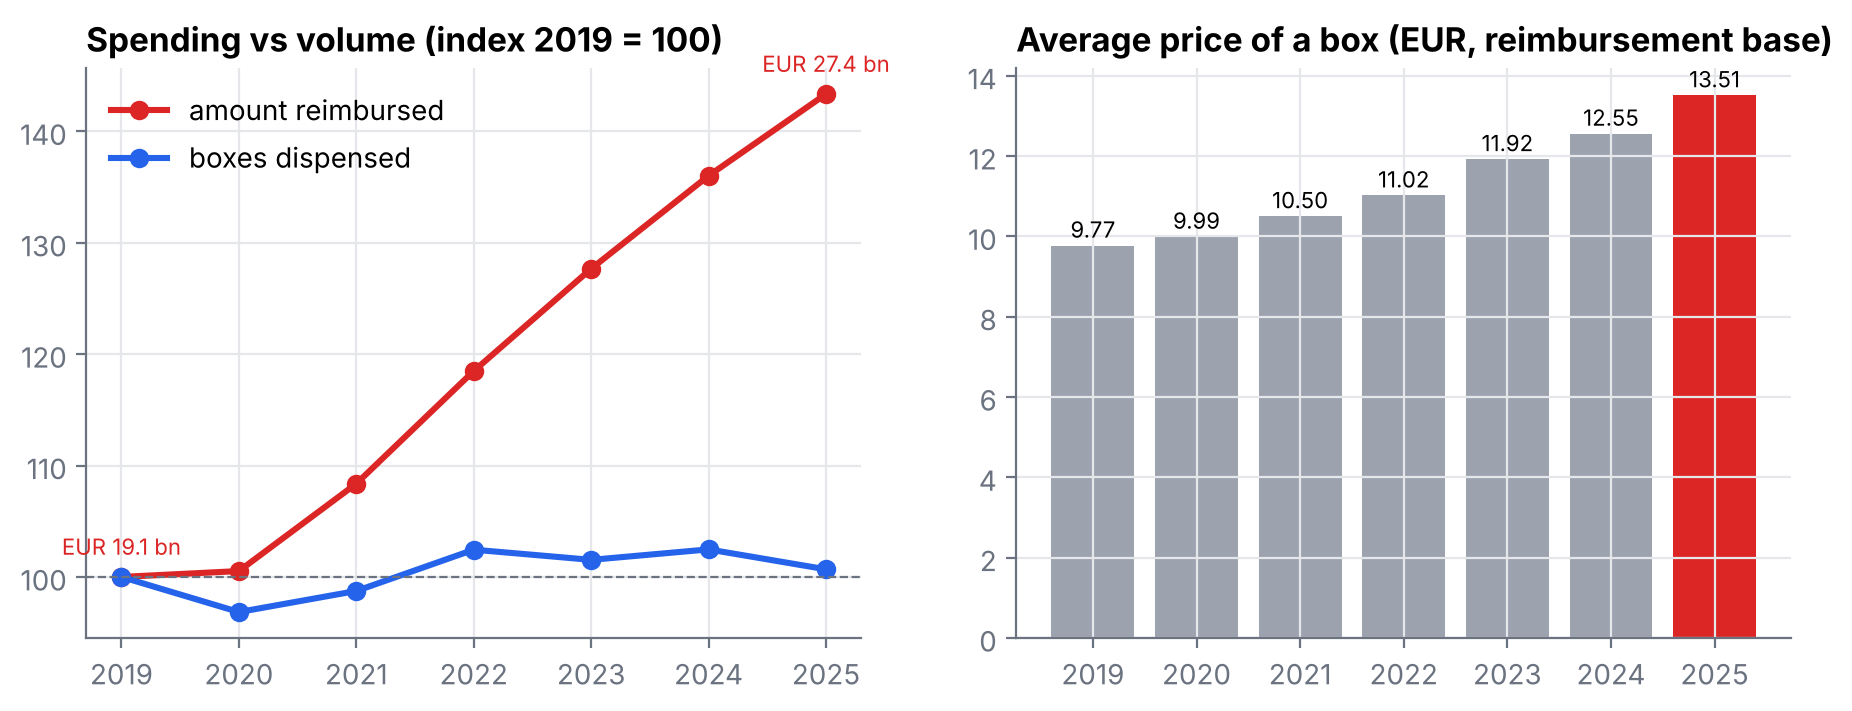
\includegraphics[width=\linewidth]{01_spending_vs_volume}\end{figure}
Apart from a pause in 2020, spending rose every year (+5 to +9\%), while the number of boxes never moved more than about 3\% from its
2019 level. The 38\% rise in the average price of a box most likely reflects new, expensive treatments replacing or adding
to cheap ones rather than price increases, since French prices of existing drugs generally fall over time; the data used
here cannot fully separate the two (see next steps).

\subsection{Where the extra \texteuro 8.3 billion went}
\begin{figure}[H]\centering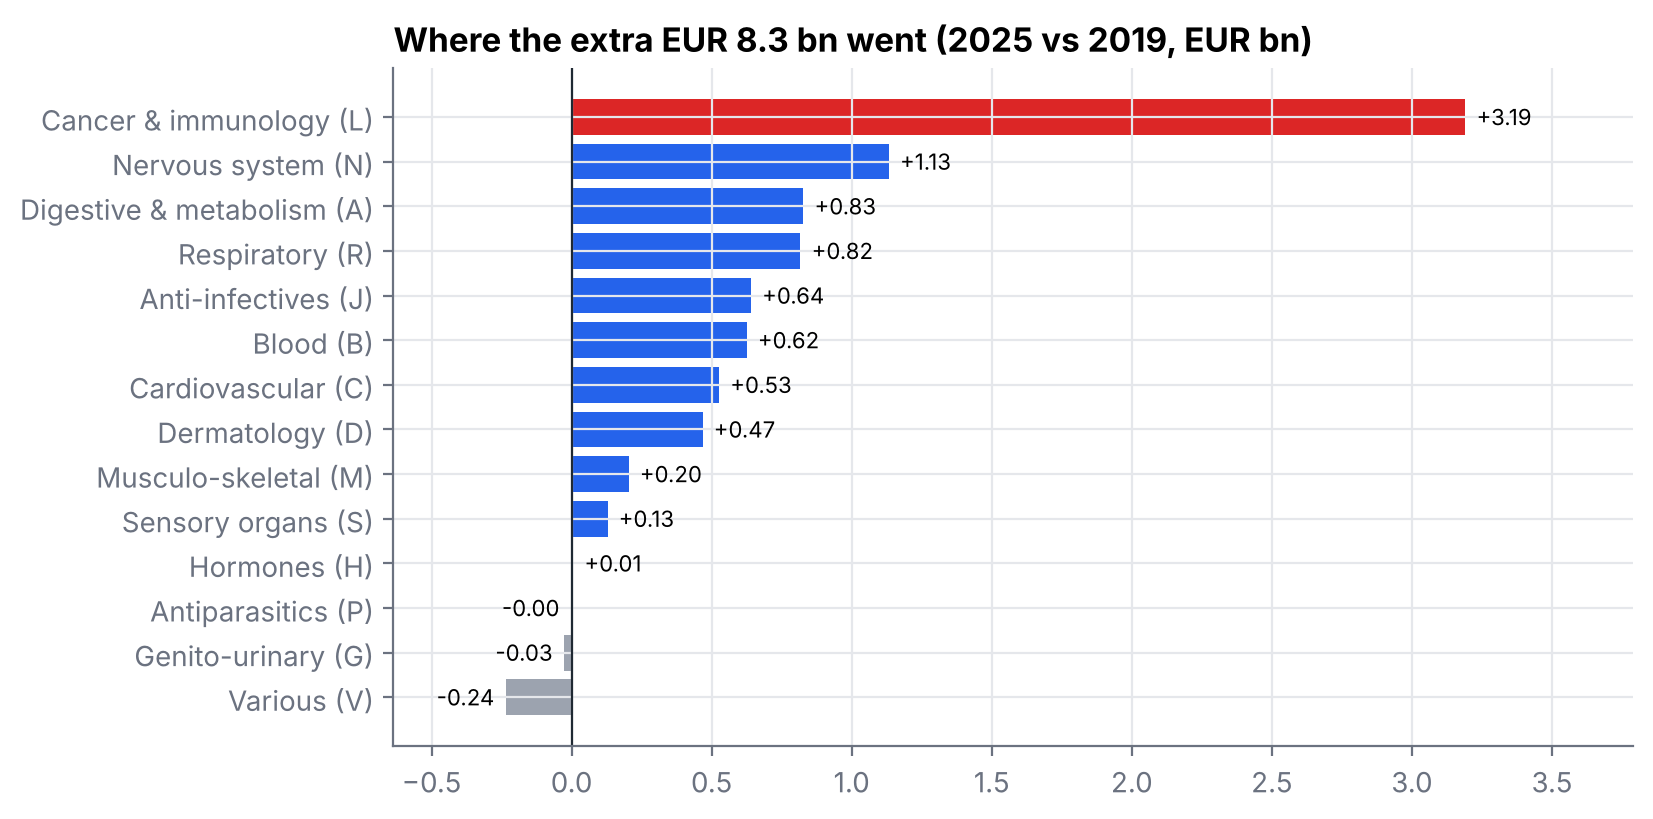
\includegraphics[width=0.8\linewidth]{02_growth_by_group}\end{figure}
Cancer and immunology (ATC group L) contribute 38\% of the growth, followed by the nervous system and metabolism. At
molecule level, the biggest increases are recent targeted therapies: tafamidis, the cystic-fibrosis triple therapy
(ivacaftor + tezacaftor + elexacaftor, from zero in 2019 to \texteuro 473 million), dupilumab (eczema, asthma),
oral cancer drugs (apalutamide, osimertinib), and diabetes or heart-failure drugs (dapagliflozin, semaglutide,
sacubitril + valsartan). The largest decreases concern drugs facing biosimilars, generics, price cuts or newer competitors (ranibizumab,
rivaroxaban, palbociclib), and liraglutide, replaced by newer GLP-1 analogues.
\begin{figure}[H]\centering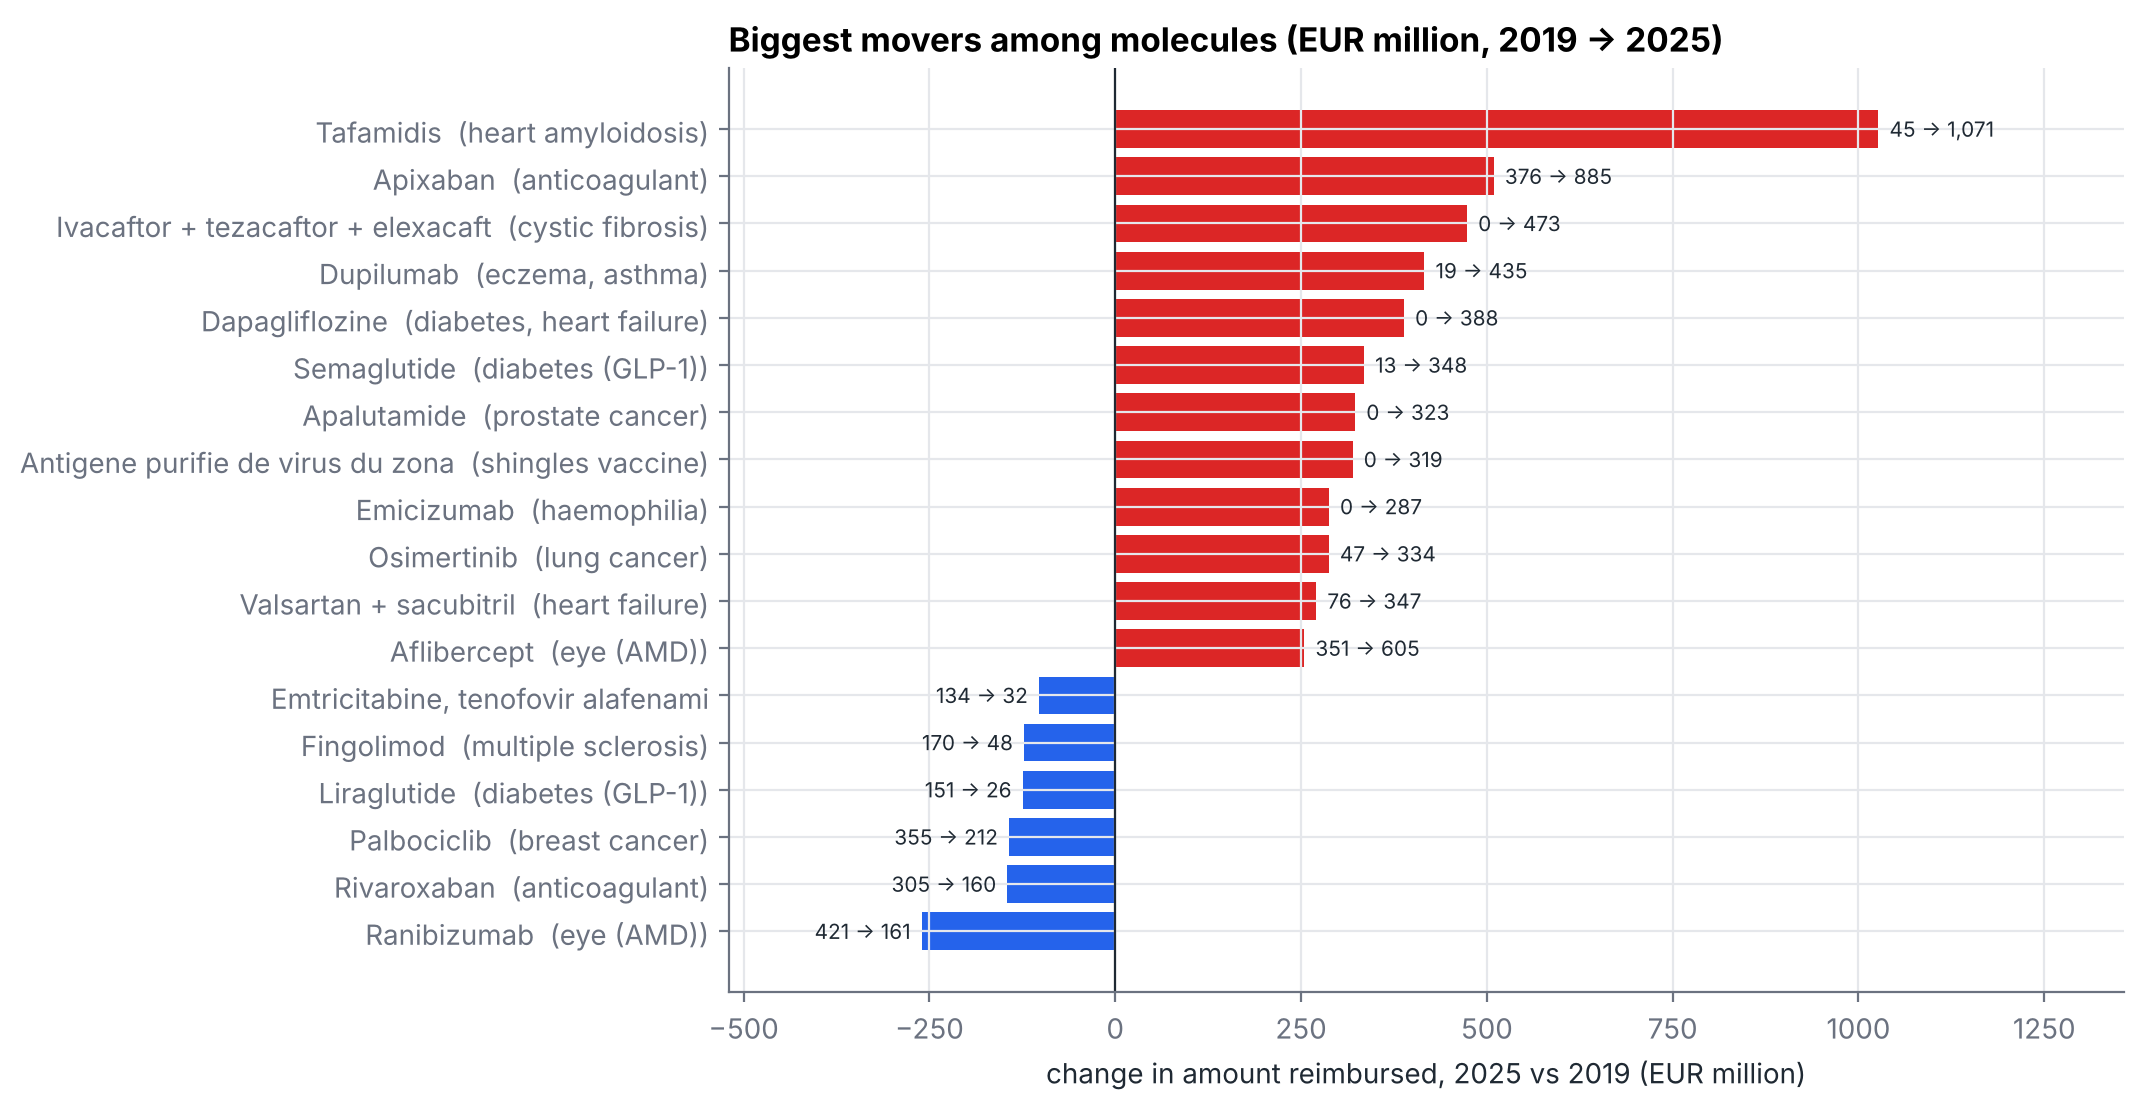
\includegraphics[width=0.9\linewidth]{03_molecule_movers}\end{figure}
\textbf{Concentration.} The 10 most reimbursed molecules weighed 17\% of spending in 2019 and 20\% in 2025; the number of
molecules making up half of spending fell from 70 to 55.

\subsection{Three shifts in medicine use}
\begin{figure}[H]\centering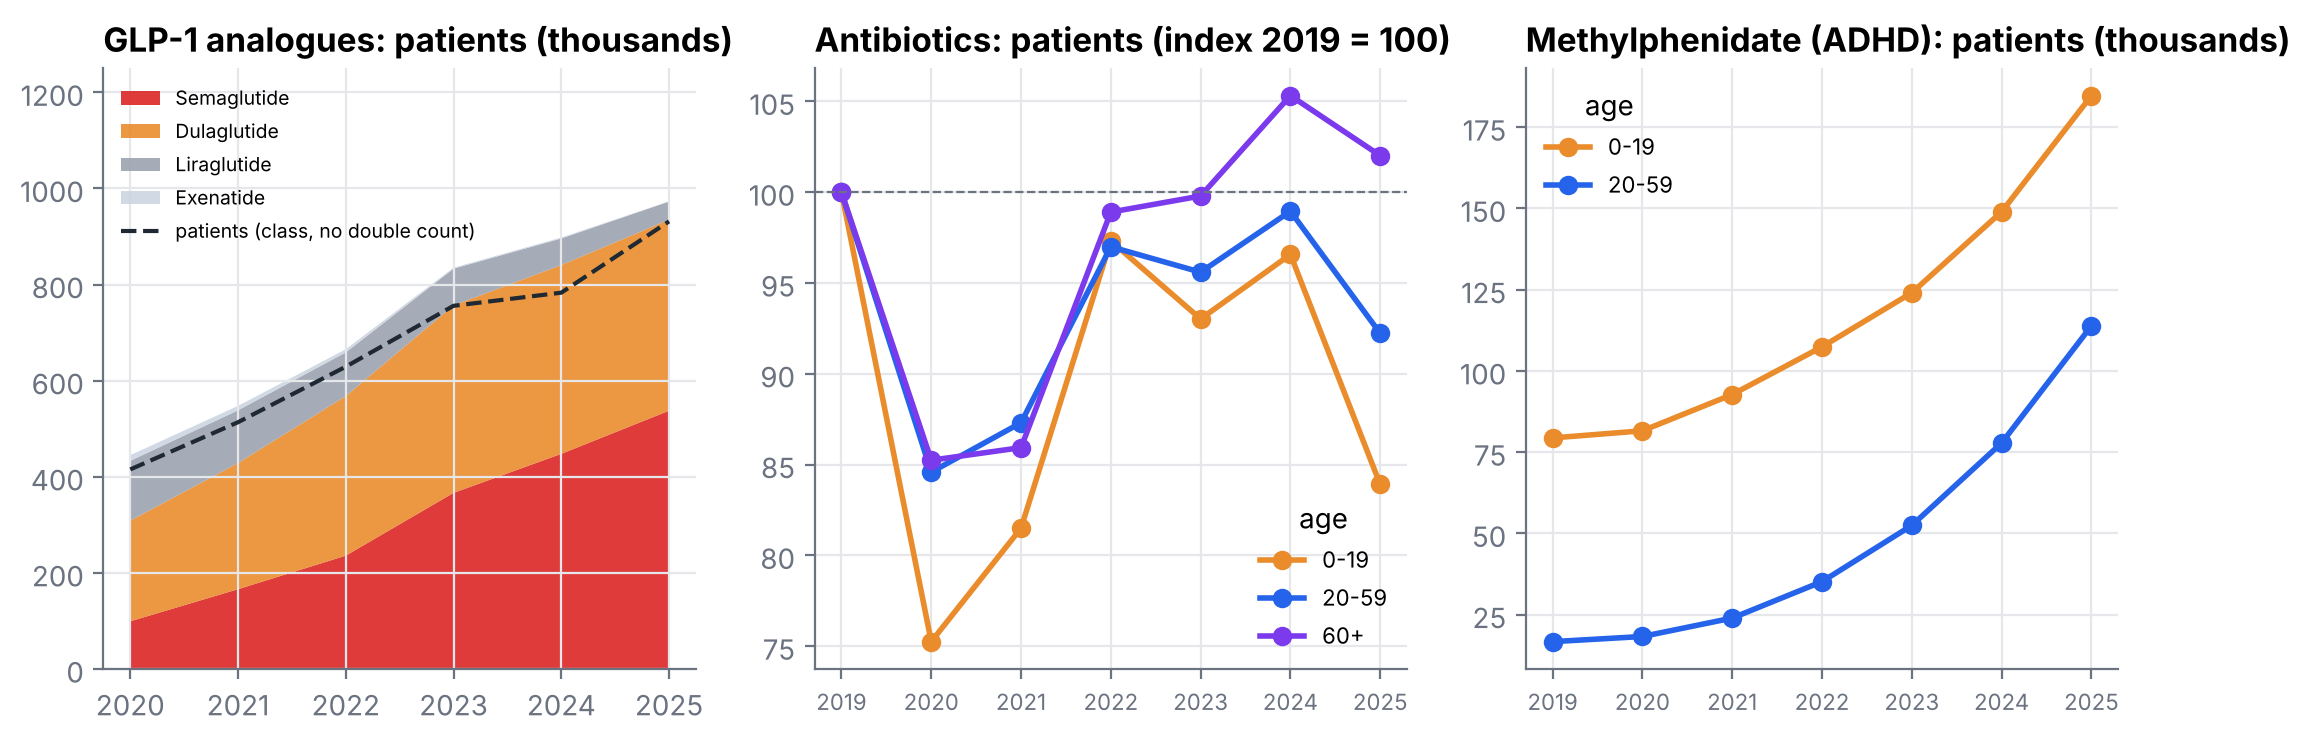
\includegraphics[width=\linewidth]{04_three_stories}\end{figure}
\textbf{GLP-1 analogues.} Patients rose from 415{,}000 (2020) to 932{,}000 (2025), and reimbursements from \texteuro 352 to
\texteuro 675 million. Semaglutide overtook dulaglutide in 2024 and reached 537{,}000 patients. 64\% of patients are
over 60 and 47\% are women. In France these drugs are reimbursed for type~2 diabetes; anti-obesity use is mostly not
reimbursed and therefore not visible here.

\textbf{Antibiotics.} In 2020 the number of patients fell by 17\% (25\% among under-20s): lockdowns, masks and distancing
cut the spread of infections. Use rebounded in 2022 and was back to its 2019 level in 2024 (28.1 million patients),
before falling again in 2025.

\textbf{ADHD.} The number of people treated with methylphenidate tripled, driven by adults: from 17{,}000 to 114{,}000
(\texttimes 6.8), while children went from 79{,}000 to 185{,}000. Adults now make up 38\% of patients.

\subsection{Regions: age explains much of the gap}
People aged 60 and over cost \texteuro 852 per inhabitant in 2025, against \texteuro 262 for 20--59 and \texteuro 110 for
under-20s; they account for 59\% of spending. Regions with older populations therefore look expensive.
\begin{figure}[H]\centering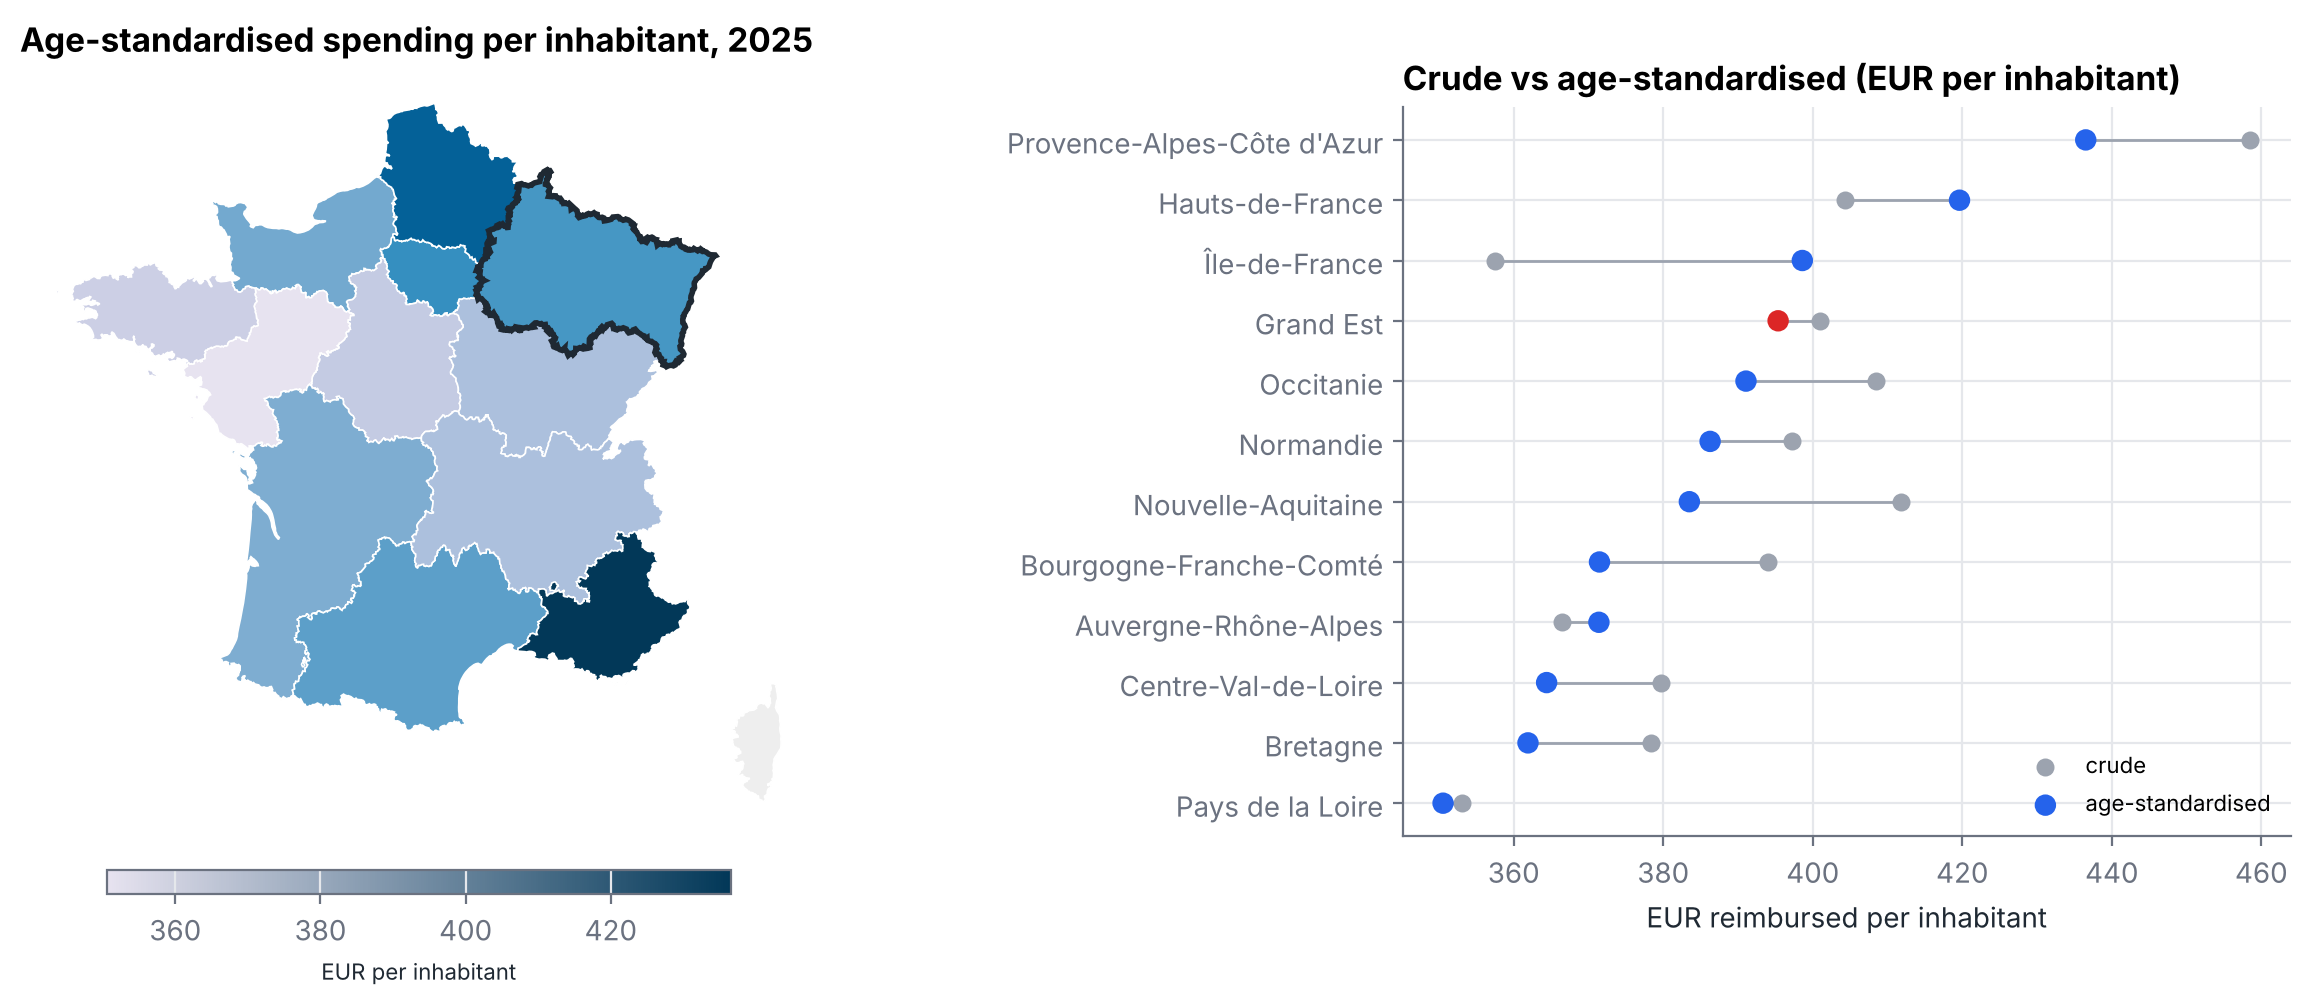
\includegraphics[width=\linewidth]{05_regions}\end{figure}
Once standardised, Île-de-France, the youngest region, jumps from 11th to 3rd (\texteuro 358 $\rightarrow$ \texteuro 399),
Nouvelle-Aquitaine falls from 2nd to 7th, and Hauts-de-France rises to 2nd, in line with its known poorer health
indicators. Provence-Alpes-Côte d'Azur stays first on both measures. \textbf{Grand Est} is 5th crude (\texteuro 401) and
4th standardised (\texteuro 395), slightly above the median of \texteuro 385.

\section{Limitations}
\begin{itemize}
  \item \textbf{Retail pharmacies only}: expensive hospital drugs (many cancer treatments) are not included, so the share of
        cancer drugs in total French drug spending is larger than shown here.
  \item \textbf{List prices}: amounts are before confidential rebates negotiated between companies and the State, which
        are large for some innovative drugs; net spending is lower.
  \item \textbf{Three age groups only}: age standardisation is coarse; within ``60+'' an 85-year-old costs far more than a
        65-year-old.
  \item \textbf{Regions}: Corsica is not published separately in Open Medic and 6.4\% of spending has no metropolitan
        region; population for 2024--2025 reuses 2023.
\end{itemize}

\section{Next steps}
\begin{enumerate}
  \item Add generic vs brand-name status (available in the detailed Open Medic base) to measure savings from generics.
  \item Split the price effect between new drugs and price changes of existing ones (a Laspeyres-type decomposition).
  \item Use prescriber specialty to see who drives the growth of GLP-1 and ADHD treatments.
  \item Forecast 2026 spending by therapeutic group.
\end{enumerate}

\section*{Reproducibility}
Code, SQL and notebook: \href{https://github.com/LDGKM/medicine-spending-france}{github.com/LDGKM/medicine-spending-france}.
\texttt{python run\_all.py} downloads the data and regenerates every table and figure.
Tools: Python, DuckDB (SQL), pandas, matplotlib. Data: Assurance Maladie (Open Medic), INSEE.

\end{document}
